\documentclass{elsarticle}

\usepackage[utf8x]{inputenc}
\usepackage[table]{xcolor}
\usepackage{amsmath}
\usepackage{amssymb}
\usepackage{url}
\usepackage{graphicx}
\usepackage[table]{xcolor}
\usepackage{tabularx}
\usepackage{multirow,makecell}
\usepackage{float,lscape}
\usepackage[ruled,linesnumbered,vlined]{algorithm2e}
\usepackage{tkz-graph}
\usepackage{lscape} 
\usepackage[binary-units=true]{siunitx}

\definecolor{gold}{HTML}{FFF3D6}
\definecolor{silver}{HTML}{F3F5F7}
\definecolor{cupper}{HTML}{EAD9D7}
\fboxsep0pt
\newcommand{\firsto}{\colorbox{gold}{\texttt{M1}}}
\newcommand{\firsts}{\colorbox{gold}{\texttt{s1}}}
\newcommand{\firstu}{\colorbox{gold}{\texttt{u1}}}
\newcommand{\firstp}{\colorbox{gold}{\texttt{P1}}}
\newcommand{\secondo}{\colorbox{silver}{\texttt{M2}}}
\newcommand{\seconds}{\colorbox{silver}{\texttt{s2}}}
\newcommand{\secondu}{\colorbox{silver}{\texttt{u2}}}
\newcommand{\secondp}{\colorbox{silver}{\texttt{P2}}}
\newcommand{\thirdo}{\colorbox{cupper}{\texttt{M3}}}
\newcommand{\thirds}{\colorbox{cupper}{\texttt{s3}}}
\newcommand{\thirdu}{\colorbox{cupper}{\texttt{u3}}}
\newcommand{\thirdp}{\colorbox{cupper}{\texttt{P3}}}


\title{SAT Competition 2020\tnoteref{title}}
\tnotetext[title]{\url{satcompetition.github.io/2020}}

\author[jku]{Nils Froleyks}
\ead{nils.froleyks@jku.at}
\author[cmu]{Marijn Heule}
\ead{marijn@cmu.edu}
\author[kit]{Markus Iser}
\ead{markus.iser@kit.edu}
\author[hiit]{Matti Järvisalo}
\ead{matti.jarvisalo@helsinki.fi}
\author[ctu]{Martin Suda} 
\ead{martin.suda@cvut.cz}

\address[jku] {
Institute for Formal Models and Verification, Johannes Kepler University\\
{\tt nils.froleyks@jku.at}\\[1em]
}


\address[cmu] {
Computer Science Department, Carnegie Mellon University\\
{\tt marijn@cmu.edu}\\[1em]
}

\address[kit] {
KIT Department of Informatics\\
{\tt markus.iser@kit.edu}\\[1em]
}

\address[ctu] {
Czech Technical University in Prague, Czech Republic\\
{\tt martin.suda@cvut.cz}\\[1em]
}


\newcommand{\todo}[1]{{\color{purple}Todo: #1}}
\newcommand{\solver}[1]{\texttt{#1}}

% Stack a variable number of arguments:
\makeatletter
\newcommand{\stack}[1]{%
\begin{tabular}{@{}l@{}}#1\checknextarg}
\newcommand{\checknextarg}{\@ifnextchar\bgroup{\gobblenextarg}{\end{tabular}}}
\newcommand{\gobblenextarg}[1]{\\#1\@ifnextchar\bgroup{\gobblenextarg}{\end{tabular}}}
\makeatother

\begin{document}

\begin{abstract}
SAT Competition 2020 stands in the tradition of the series of annual competitive events which motivate and assess the progress in SAT solving. 
This competition was special as it introduced the new cloud track where SAT Solvers that run on hundreds of processors could compete. 
Another novelty was the application-specific sub-track of the main track, 
where solvers competed in solving benchmark instances from one specific domain only, and in this year that was the planning domain. 
We used new tools to select and distribute benchmark instances and their attributes. 
In this paper we provide a description of the well-known and the new competition tracks and how we organized them. 
It follows then a detailed analysis of the results and the strategies of the award winning solvers. 
\end{abstract}

\begin{keyword}
SAT, Competition
\end{keyword}

\maketitle

\section{Introduction}

Propositional satisfiability (SAT) is the archetypal NP-complete problem. 
Despite its complexity, there is ongoing progress in solving methods and their implementations in SAT solvers. 
The generic nature of the SAT problem as well as the performance of state-of-the-art SAT solvers facilitate their use as the algorithmic backend in a plethora of applications. 
Today, SAT solvers are used for verification of hard- and software, product configuration, cryptography, planning and scheduling, to name a few. 
In mathematics, SAT solvers were recently even used to generate a record sized proof (200 TB) for an until then unsolved problem in Ramsey theory. 

SAT Competitions are organized regularly since 1992 in order to drive progress and to serve as a public assessment of the state-of-the-art in SAT solving. 
For each SAT Competition, a set of new benchmark instances is compiled which reflects the various applications of interest to the community. 

In this competition, we initiated a new application-specific subtrack. 
The idea is to provide a large amount of benchmark instances of a specific application, and to evaluate all solvers with respect to these instance in a special track. 
In this competition, we used 200 instances of the planning domain to run a planning subtrack. 

Faster networks, distributed systems, and the increasing number of processors in modern computers show that the trend of increasing parallelism is about to continue.  
In the new cloud track, for the first time, solver authors could compete in SAT technologies that allow hundreds of SAT solvers to cooperate in solving a SAT instance. 

\todo{Present some important pointers for SAT and CDCL}

In Section~\ref{sec:overview}, we start with an overview of the competition,
including detailed description of the competition tracks and their purpose,
the general rules and the used computing environment.
Section~\ref{sec:instances} contains an overview on the selected benchmark instances and details about the selection process. 
In Section~\ref{sec:results}, we present the competition results alongside a survey on the winning strategies of the award winning solvers. 
A meta-analysis of these results follows in Section~\ref{sec:analysis}, and we conclude with Section~\ref{sec:conclusion}.

\todo{maybe mention \url{https://satcompetition.github.io/2020/}}

\todo{Maybe mention proceedings \cite{SC2020}}

\section{Overview of the Competition}
\label{sec:overview}

In this section, we describe the individual 2020 SAT Competition tracks,
explain the requirements for participation % input/output and proof formats,
and the ranking criteria, as well as
the computing infrastructure used for executing the competition.

\subsection{Competition Tracks}

SAT Competition 2020 consisted of four tracks:
the Main track, Incremental Library track, Parallel track,
and the Cloud Track for massively parallel SAT solvers using up to 1024 cores. 
Furthermore, the Main track comprised of several sub-tracks.

\subsubsection{Main Track}

The focus of the traditional Main track is on sequential SAT solvers and their evaluation on structured, non-random benchmarks coming from various application areas. To participate in the main track, solvers needed to output certificates both for the satisfiable and the unsatisfiable answer. Moreover, the source code of the solver had to be made publicly available. 

Solvers not complying with either of the above criteria were only evaluated in a so-called No-Limits sub-track and were not eligible for the Main track awards. The No-Limits thus enabled participation of closed-source solvers (not being able or willing to expose the source code for legal or other reasons) as well as portfolio solvers (combining two or more core SAT solvers developed by different groups of authors; c.f.~Sect.~\ref{sec:rules}). However, solvers in No-Limits still competed against all other solvers in the Main Track (hence, we consider it a sub-track). The No-Limits sub-track was only evaluated with respect to the benchmarks instances which were \emph{newly} submitted to SAT Competition 2020.

Part of the Main track was the Planning sub-track, in which we evaluated the solvers on 200 benchmarks 
which all came from the same application domain -- automated planning. 
Solver submitted to the Main track automatically participated in the Planning sub-track.
It is envisioned, that also in the future there will be an application sub-track of the Main track, each time highlighting a different area where the SAT solving technology helps to advance the state of the art.

Finally, the Main Track also had the so-called ``Glucose hack'' sub-track. 
Since in the past several advances in SAT solving required only a small modification of an established solver
to achieve a considerable contribution, this sub-track encouraged participation 
of small modifications of the Glucose 3.0 SAT solver. The limit for being considered a ``hack''
was set to 1000 non-space character edit distance from the sources of Glucose provided by the organisers. 
Unfortunately, in 2020 there were not enough participants in this sub-track and we do not report on it 
in the results section.

\subsubsection{Incremental Library Track}

In the Incremental Library track we mimic scenarios
where a SAT solver is used as a backend solver in a more complex tool
(typically solving a harder problem than SAT) and is called multiple times before 
the enclosing tool reaches its final state. Incrementality means that
the individual calls to the SAT solver are not independent, but may share 
a common subset of the input clauses or differ in the presence of additional 
unit clause assumptions~\cite{Nadel:2014:Incremental,Fazekas:2019:IncrementalInprocessing}. 

Instead of using or extending the DIMACS input format, we realize the Incremental track
by relying on the general incremental interface IPASIR (Re-entrant Incremental Solver API) 
for SAT applications~\cite{Balyo:2015:SATRace}. The idea is that we actually run the 
enclosing tool on its own benchmark and communicate with the competing SAT solver 
through this interface API. Not only does the SAT solver in this track
need to solve a sequence of related problems fast, but its answers to the early questions
may in general influence which questions will follow next.
% E.g. Smaller unsat cores may allow the enclosing tool to converge using fewer SAT calls!

\subsubsection{Parallel Track}

\todo{MH?}

\subsubsection{Cloud Track}

\todo{MH?}

\subsection{Mandatory Participation Requirements}
\label{sec:rules}

The following requirements were imposed for 
the participation in the competition.

\paragraph{Source Code}
The source code of submitted SAT solvers had to be made available 
(licensed for research purposes) except for the solvers participating only in the No-Limits sub-track.

\paragraph{Description}
A short system description was required for each solver submission,
including a list of all the solver's authors and explaining any non-standard algorithmic
techniques and data structures, as well as references to the relevant literature.
These system descriptions have been collected and published in the competition
proceedings \cite{SC2020}.

\paragraph{Benchmarks}
To participate in the Main track, each team had to submit 20 new benchmark instances.
This rule guaranteed that the competition could be run on instances mostly unseen to the solver
developers prior to the competition. Moreover, by making these benchmarks publicly available
after the competition, the SAT community benefits by having an ever growing repository 
of diverse problems to target with the next developments.

The exact details of this rule are further explained in Section~\ref{sec:byob}.
Also the descriptions of the benchmarks have been published \cite{SC2020}.

\paragraph{Input and Output Format}

The benchmark instances were presented to the solvers in the de facto standard
DIMACS input format for propositional formulas in conjunctive normal form.
A simple extension of this format was to be adhered to when printing 
the satisfying assignment 
(see, e.g., \cite{DBLP:journals/jsat/HeuleJS19}, Section 2.4).

Proofs of unsatisfiability were to be emitted in the DRAT format~\cite{DRATtrim},
either in its textual version, which is also very similar to the DIMACS input format,
or on a more compact binary version (for more details, see \cite{satComp2020www}, Unsat Certificates).
%
Details on certification are further discussed below in Section~\ref{sec:certif}.

\paragraph{Number of submissions}

Each participant was restricted to be an author of at most four different sequential solvers,
two different parallel solvers, and one ``Glucose hack'' sub-track solver.
Two solvers were considered different as soon as their sources differed
or the compilation options were different, or different command line options were used
(with the exception of an option enabling or disabling the proof output).

\paragraph{Portfolio Solvers}

Apart from the No-limits sub-track, participants were not allowed to submit a portfolio of solvers,
i.e., a combination of two or more core SAT solvers developed by different groups of authors.\footnote{
In other words, a submission of a combination of solvers was only possible if all the authors of all the parts
were explicitly listed. This means that all the authors had to be notified if such participation
was planned and had to consider it carefully, also taking into account the limited number of submissions per author
as specified by the previous rule.}

This rule is mainly meant to encourage the SAT community to invest more effort into developing new solver code bases.
Moreover, while acknowledge that research on solver selection tools that typically orchestrate portfolio solvers 
is interesting, it is not the focus of the SAT competition.

\todo{Should we have a discussion (maybe in later sections)
about the future of the portfolio solver rule
concerning the point raised by Mate Soos (in emails)?}

\paragraph{Organizers}
The organizers of the competition were not allowed to participate.

\subsection{Solver Ranking and Disqualification}

Solvers were ranked using a PAR-2 score based on a \num{5000}-second timeout.
A PAR-2 system assigns as many points as the number of seconds it took the solver
to solve a particular instance and twice the time limit, i.e.~\num{10000} points,
if the instance was not solved. This means that lowers scores are better.
We generally report the average score of each solver
across a benchmark set.

A SAT solver was disqualified if it produced a wrong answer. 
Specifically, if a solver reported ``unsatisfiable'' on an instance that 
was proven to be satisfiable by some other solver, or reported ``satisfiable'' 
but provided a wrong certificate. Solvers disqualified from the competition were
not eligible to win any award. 

\subsection{Certificates}

\label{sec:certif}

In all tracks it was required to output a model to certify recognising a satisfiable instance.
On the other hand, certificates for unsatisfiable instances (proofs) were required only 
in the Main track (besides the No Limits sub-track).

The proofs were validated in a two step fashion. First, the tool {\tt DRAT-trim}~\cite{DRATtrim}
was used for initial checking and optimizing the emitted proof, deriving a so-called LRAT proof file.
Afterwards, an independent, formally-verified checker {\tt cake\_lpr} \cite{cakeLprGithub}, 
was used for validating the LRAT proof as a correct proof of unsatisfiability of the given formula.
In the Main track, we only considered solved those unsatisfiable formulas that 
could be validated by {\tt DRAT-trim}.
There were several cases where {\tt cake\_lpr} ran out of resources before being able to 
confirm after {\tt DRAT-trim}. However, there was no case where {\tt DRAT-trim} would accept
a proof and {\tt cake\_lpr} would later disagree with the verdict.

\subsection{Computing environments}

\label{sec:computing}
The Main Track with its sub-tracks was run on the StarExec cluster \cite{starexec},
whose nodes are equipped with Intel Xeon \SI{2.4}{\giga\hertz} processors 
and \SI{128}{\giga\byte} of memory.
The time limit enforced on each solver for solving an instance was \SI{5000}{\second}. 
(In the Main track, validation then continued for up to \SI{45000}{\second}.)
The solvers were allowed to use up to the full \SI{128}{\giga\byte} of RAM.\footnote{
Unfortunately, the memory limit of \SI{24}{\giga\byte}, that was used in the previous years,
was by mistake advertised on the competition web page prior to solver submission.
This could have resulted in some solvers not ``daring'' to use the full \SI{128}{\giga\byte}
in the competition.}

The Incremental Library Track was run on computers with 2x Intel Xeon E5430 \SI{2.66}{\giga\hertz}
(4-Core) processors and \SI{24}{\giga\byte} of RAM.

\todo{Parallel / Cloud}

\section{Description of Benchmark Instances}
\label{sec:instances}

For selection of benchmark instances in this competition, we used GBD Tools.%
\footnote{\url{https://pypi.org/project/gbd-tools/}} 
Using the concept of instance identification via GBD Hash, which is the hash-sum of the unpacked and normalized DIMACS file, GBD Tools provide utilities to query for instances with desired properties, e.g., instance author, family and result.
The association of instance-id and instance attributes is maintained in publicly available databases.%
\footnote{\url{https://gbd.iti.kit.edu}}

GBD Tools is a tool-chain for maintenance and distribution of benchmark instances and instances features~\cite{Iser:2018:GBD}. 
Its databases provide information about all instances used in SAT competitive events dating back to 2006. 
In GBD Server, each instance also has an URL, such that instances can be distributed by using their identifier: \url{https://gbd.iti.kit.edu/file/<gbd-hash>}.


\subsection{Selection of Instances}
\label{sec:byob}

\begin{algorithm}[t]
\DontPrintSemicolon

\KwData{$I$ : Set of Instances, $A$ : Set of Authors}
\KwData{Functions $\alpha : I \rightarrow A$ and $\sigma : I \rightarrow \{\mathsf{sat}, \mathsf{unsat}, \mathsf{unknown}\}$}
\KwResult{$S$ : Set of Selected Instances}
\SetKwFunction{rand}{$\mathsf{random.choice}$}
\BlankLine
$S \leftarrow \emptyset$\;

\For {$a \in A$} {
	$I_a^+ \leftarrow$ \rand{$\{ e \in I \mid \alpha(e) = a \land \sigma(e) = \mathsf{sat} \}$, $k=7$}\;	
	$I_a^- \leftarrow$ \rand{$\{ e \in I \mid \alpha(e) = a \land \sigma(e) = \mathsf{unsat} \}$, $k=7$}\;	
	\If {$|I_a^+|+|I_a^-| < 14$}{
		$l \leftarrow 14 - (|I_a^+|+|I_a^-|)$\;
		$I_a^? \leftarrow$ \rand{$\{ e \in I \mid \alpha(e) = a \land \sigma(e) = \mathsf{unknown} \}$, $k=l$}\;
	}
	$S \leftarrow S \cup I_a^+ \cup I_a^- \cup I_a^?$\;	
}
\Return $S$\;

\caption{Benchmark Instance Selection}
\label{algo:select}
\end{algorithm}

\begin{table}[t]
\small
\centering
\begin{tabular}{|l|l||rr|}
\hline
Family & Author & Submitted & Selected\\
\hline\hline
0-1 Integer Programming & Riveros & 6 & 2 \\
Anti-Bandwidth & Biere & 187 & 14 \\
Baseball Lineup & Hickey & 40 & 13 \\
Bit-Vector & Preiner & 393 & 14 \\
Cellular Automata & Chowdhury & 20 & 12 \\
CNF Miter & Manthey & 38 & 7 \\
Coloring & Oostema & 14 & 14 \\
Core-based Generator & Hartung & 20 & 14 \\
Cover & Gacek & 18 & 13 \\
Cryptography & Paxian, Shaw, Soos & 106 & 34 \\
Discrete Logarithm & Jingchao & 20 & 7 \\
Edge Matching & Holten & 58 & 7 \\
Fermat & Riveros & 8 & 5 \\
Flood-It Puzzle & Stiphout & 40 & 0 \\
HGen & Guanfeng & 20 & 13 \\
Hypertree Decomposition & Schidler & 56 & 14 \\
Influence Maximization & Kochemazov & 20 & 14 \\
Lam Discrete Geometry & Nejati & 20 & 9 \\
Polynomial Multiplication & Maoluo & 20 & 8 \\
Schur Coloring & Riveros & 4 & 2 \\
Station Repacking & Newman & 20 & 12 \\
Stedman Triples & Johnson & 23 & 7 \\
Sum Subset & Riveros & 5 & 2 \\
Tensors & Savicky & 20 & 14 \\
Termination & Yolcu & 12 & 7 \\
Timetable & Djamegni & 20 & 14 \\
Tournament & Heule & 16 & 14 \\
Vlsat & Bouvier & 36 & 14 \\
\hline
\multicolumn{2}{|r||}{$\Sigma$} & 1260 & 300 \\
\hline
\end{tabular}
\caption{Families and amounts of newly submitted instances}
\label{tab:families}
\end{table}

The ``Bring Your Own Benchmarks'' (BYOB) rule is established since SAT Competition 2017~\cite{SC2017}. 
By this rule solver authors are required to submit $20$ new benchmark instances in order to participate in the competition. At least $10$ of these instances are required to be ``interesting'', meaning that Minisat must need more than a minute to solve it and the authors own solver does not run into a timeout for the instance. 

As can be seen in Table~\ref{tab:families}, a total of $28$ authors followed our calls for participation and benchmark instances, thus contributing a set of $1260$ previously unseen benchmark instances in a large variety of different instance families. 

By filtering out instances with could be solved by Minisat in less than $10$ minutes, we obtained an initial set of $1012$ instances. 
In order to compile a balanced set of $300$ benchmark instances, we considered a maximium of $14$ submissions per author and used the procedure which is depicted in Algorithm~\ref{algo:select}. 
Per author, if possible, we first randomly selected $7$ satisfiable and $7$ unsatisfiable instances (lines~3 and~4). 
If this did not yield a total of $14$ instances, we added instances of yet unknown outcome (lines~5-7). 
Of the such obtained $308$ instances, we randomly removed $8$ satisfiable instances, yielding a total of $114$ satisfiable, $78$ unsatisfiable and $108$ instances of unknown result. 

To obtain the final compilation of $400$ benchmark instances, we augmented this set with $100$ instances which have been used in previous competitions. 
We randomly selected $21$ satisfiable, $57$ unsatisfiable and $22$ unknown instances to yield a total of $135$ satisfiable, $135$ unsatisfiable and $130$ instances of unkown result. 
Furthermore, we made sure not to select instances of a family which is already represented in the set of newly submitted instances and excluded random, agile and planning instances (due to the planning track). 

Table~\ref{tab:families} displays the numbers of submitted and selected instances grouped by problem family and author. 

\begin{table}[t]
\centering
\begin{tabular}{|r|ccc|c|}
\hline
 & SAT & UNSAT & UNKNOWN & $\Sigma$\\
\hline\hline
New Instances & 114 & 78 & 108 & 300 \\
Old Instances & 21 & 57 & 22 & 100\\
\hline
$\Sigma$ & 135 & 135 & 130 & 400\\
\hline
\end{tabular}
\caption{Amount of old and new instances by result}
\label{tab:final}
\end{table}


\subsection{Planning Instances}
Classical planning is the problem of finding a sequence of actions -- a plan --
that transforms the world from some initial state to a goal state. In 1992 Kautz
and Selman
\cite{Kautz1992} proposed to encode planning as satisfiability. In their
encoding the problem of finding a plan of length $i$ (\textit{i.e.,} the
\emph{makespan}) is translated into a Boolean formula $F_i$ that is satisfiable
exactly if a plan of length $i$ \emph{or less} exists. In later encodings
multiple actions can be executed \emph{in parallel} allowing longer plans to be
found by solving smaller formulas \cite{Rintanen2006, Rintanen2007, Balyo2013}.

Finding the minimal makespan $i$ for which $F_i$ is satisfiable is important for
SAT-based planning in general and the generation of this benchmark set in
particular. The minimal makespan depends on the planning task and the used
encoding. The hardest formulas that a SAT-based planner has to solve are usually
the last unsatisfiable $F_i$ before the next higher makespan becomes satisfiable
\cite{Rintanen2006}. Therefore we preferably pick the last unsatisfiable
makespan for each planning task to generate unsatisfiable instances. For
planning tasks where this makespan cannot be determined with available
computational resources, we use a \emph{sequential} encoding, where the minimal
makespan equals the length of the shortest valid plan. Together with known
bounds\footnote{Bounds on plan length are available for some planning tasks from
  the \emph{optimal track} that have \emph{unit cost} actions.} on the optimal
plan length we can generate SAT formulas with predetermined satisfiability for
hard planning problems.

The encodings are generated by the two SAT-based planners \emph{Madagascar}
\cite{Madagascar14} and \emph{Pasar} \cite{Pasar19}. We use Madagascar both in
its default configuration to generate a parallel encoding based on
$\exists$-step plans and to generate the sequential encoding where needed. Pasar
uses the \emph{grounding routine} deployed by the well known planner \emph{Fast
  Downward} \cite{FastDownward06} to translate planning tasks into a different
formalism and then encodes it to SAT using a parallel encoding.

The classical planning benchmarks are selected from the \emph{satisficing} and
\emph{optimal} tracks of the \emph{International Planning Competitions} 2014
\footnote{\url{https://helios.hud.ac.uk/scommv/IPC-14/repository/benchmarksV1.1.zip}}
and 2018 \footnote{\url{https://bitbucket.org/ipc2018-classical/domains}}.

In addition to the classical planning problems, we also include SAT formulas
generated by \emph{Tree-REX} \cite{TreeRex19}; a planner for \emph{Hierarchical
  Task-networks}. In HTN planning the planner is provided with additional domain
knowledge besides the problem description. The HTN benchmarks are provided by
the author of \emph{Tree-REX}.

Table \ref{tab:planningBenchmarkDist} shows the number of benchmarks generated
by each encoding.

\begin{table}[h]
  \caption{Number of benchmarks generated by each encoding.}
  \centering
  \begin{tabular}{@{}|l@{\hspace{3pt}}|l|r|r|@{}}
    % &Encoding& SAT & UNSAT\\
    \hline
    \multicolumn{2}{|@{}l|}{Encoding} & SAT & UNSAT\\
    % \midrule
    \hline
    \textbf{H}  & Tree-REX & 15 & 11\\
    \textbf{P}  & PASAR & 14 & 14\\
    \textbf{ME} & Madagascar $\exists$-step & 5 & 10\\
    \textbf{MS} & Madagascar sequential & 66 & 65\\
    % \midrule
    \hline
    && 100 & 100\\
    % \bottomrule
    \hline
  \end{tabular}
  \label{tab:planningBenchmarkDist}
\end{table}

The benchmarks of the planning track adhere to the naming convention below.
For
% more details and
a complete list of the encoded planning tasks we refer to the
generation script {\color{red}BROKEN LINK}.

${\langle \texttt{SAT/UNSAT} \rangle\_\langle \texttt{encoding} \rangle\_\langle
  \texttt{pathToInstance} \rangle\_\langle \texttt{makespan}
  \rangle\text{.cnf}}$

\subsection{Incremental Library Applications and Instances}

The incremental library track was first introduced in SAT~Race~2015 and 
then took place again in SAT~Competitions 2016 and 2017. 
Benchmarks for the incremental track are divided into two parts: 
Applications which implement and use an incremental SAT solver in their backend and benchmark instances which serve as input to these applications. 
For evaluating the incremental library track of this competition, we used six applications which implement the IPASIR interface -- ranging from determination of backbone variables to SAT-based planning. 
For each of those applications, we individually selected $50$ problem instances serving as input for the respective application. 

\paragraph{Backbone Variables}

The application \textsf{genipabones} incrementally determines backbone variables in a given satisfiable SAT instances using the dual rail encoding of the given instance~\cite{Balyo:2015:SATRace}.
Backbone variables have the same value in all models of a formula~\cite{Janota:2015:Backbones}. 
We selected $50$ of the smallest and easiest satisfiable instances from previous SAT competitions to evaluate solver performance with this application. 

\paragraph{Essential Variables}

The application \textsf{genipaessentials} incrementally determines essential variables in a given satisfiable formula~\cite{Balyo:2015:SATRace}. 
Essential variables have to be assigned in all partial models of a formula~\cite{Bryant:1987:Essentials}. 
We used the same $50$ easy satisfiable instances as in backbone detection to evaluate solver performance with this application. 

\paragraph{Longest Simple Paths (LSP)}

The application \textsf{genipalsp} determines longest simple paths in a graph~\cite{Balyo:2019:LSP}. 
We selected $50$ easy LSP instances for our evaluation.\footnote{\url{http://algo2.iti.kit.edu/kalp/}} 

\paragraph{Maximum Satisfiability (MaxSAT)}

The application \textsf{genipamax} solves partial MaxSAT problems by augmenting soft clauses with activation literals which are then input to a cardinality constraint~\cite{Philipp:2015:PBLib}. 
The MaxSAT problem is then solved by incrementally minimizing the bound of that cardinality constraint. 
For this application, we selected $50$ instances from \texttt{MaxSAT Evaluation 2019}.\footnote{\url{https://maxsat-evaluations.github.io/2019/}}

\paragraph{Quantified Boolean Formulas (QBF)}
\textsf{Ijtihad} is a QBF solver which uses counter\-example-guided expansion to incrementally solve a given QBF instance with a SAT solver~\cite{Bloem:2018:QBFSAT}. 
Here we used $50$ instances from \texttt{QBF Evaluation 2019}.\footnote{\url{http://www.qbflib.org/qbfeval19.php}}

\paragraph{Planning (SAS+)}
We selected $50$ planning instances to evaluate incremental SAT solvers with \textsf{Pasar} -- a planner which uses counter\-example-guided abstraction refinement (CEGAR)~\cite{Froleyks:2019:Pasar}. 


\section{Competition Results}
\label{sec:results}

\todo{New Codebases}

\todo{Winners and Runtime Plots for all the tracks}

\subsection{Planning Sub-Track}
% - 86 out of 100 biggest (number of clauses) are planning
% - 109 / 200 in the planning track are not solved by any solver
    % - 186 / 600 in total
% - all 200 above 90\% binary clauses and half have above 99%
The instances of the planning sub-track are big compared to the rest of the
main track. Using the number of clauses as a metric; out of the $100$ biggest
instances
% of the main-track
$86$ belong to the planning track. The large size can mainly be attributed to
binary clauses. On average, more than $98$\% of the clauses are binary for
planning instances, where the average for the rest of the instances from the
main track is below $60$\%.

Despite the large size, only a few instances directly caused memory problems for
more than just a few solvers. In most cases the \SI{128}{\giga\byte} of RAM
available were sufficient.
% The saving grace might have been
% This can be attributed to
% the \SI{128}{\giga\byte} of RAM available to each solver.
However, the three biggest instances from the \emph{childsnack} family of
planning problems encoded with the \emph{hierarchical} planner \emph{Tree-REX}
caused over half of the solvers to abort with some error message related to
memory. Other solvers were still able to solve the same instances within $300$
seconds.

\subsection{Similarity of Solvers}
To investigate how similar the solvers of the main track are to each other, we
define a similarity metric based on the measured runtimes. For that we first
remove $186$ benchmarks from the collected data that have not been solved by any
solver. For the rest of the benchmarks we use the PAR-2 score,
% based on the \num{5000}-second timeout
i.\,e., for each solver we set a score of \num{10000} for unsolved instances.
This leaves us with $414$ floats
$S_{1},\dots,S_{n}$ for each solver $S$. The similarity for two solvers $A$
and $B$, normalized to the interval $[0,1]$ is defined
% as:
by Equation~\ref{eq-similarity}.

\begin{equation}
\label{eq-similarity}
	similarity(A, B) =\quad 1 - \frac{\sum{|A_{i} - B_{i}|}}{414 \cdot 10000}
\end{equation}
We calculated the \emph{similarity} between the $30$ solvers which achieved the
best PAR-2 score in the main track. The results are displayed in
Figure~\ref{fig-similarity-main} as a \emph{heat map}. Additionally the result
of hierarchically clustering the solvers based on their similarity is
illustrated as a \emph{dendrogram}. The height at which two solvers or clusters
are joined reflects how similar they are. For example
enabling the \emph{trail saving} in \emph{CaDiCaL-alluip} has no impact on the
runtime, resulting in a similarity above \num{0.999}. Thus the two solvers are joined very low in the dendrogram.
% A similar visualization was used in the SAT Challenge 2012 \todo{cite}. They used

One big cluster we can identify are the \emph{Mapel} decedents in the lower left
corner, all of which are modifications of the winners of the SAT Competition
2018 and the SAT Race 2019. \todo{I think... also race vs competition? Sorry I am new
  here NF} The solver \emph{mergesat} does not quite fit into the cluster and
has a comparatively high similarity to the \emph{CryptoMiniSat} (\emph{CMS})
family at the top right. With the exception of \emph{mergesat} and maybe
\emph{DurianSat} we observe a high similarity within the cluster.

The three \emph{Relaxed} solvers by \emph{Zhang} and \emph{Cai} are using the
same code base as a lot of the solvers in the Maple-Cluster but their overall
performance is better and closer to the CMS-Cluster.

The CMS versions differ in their implementation of stochastic local search (SLS)
but overall have a similar performance.

The last big cluster in the center of the heat map is comprised of the solvers
originally written by Biere. The three configurations of \emph{Kissat} form a
subcluster, even though the configurations are fairly distinct from each other.
% , specialized for satisfiable and unsatisfiable instances.
% One targets satisfiable instances, while the other is focused on unsatisfiable
% instances and a third alternating between them.

The other subcluster consists of
modifications to the 2019 version of \emph{\mbox{CaDiCaL}}. The new version
CaDiCaL-2020 has a worse overall performance than
% has an overall worse per
% is lacking behind
the other solvers in this cluster.

\begin{figure}[tp]
    \centering
    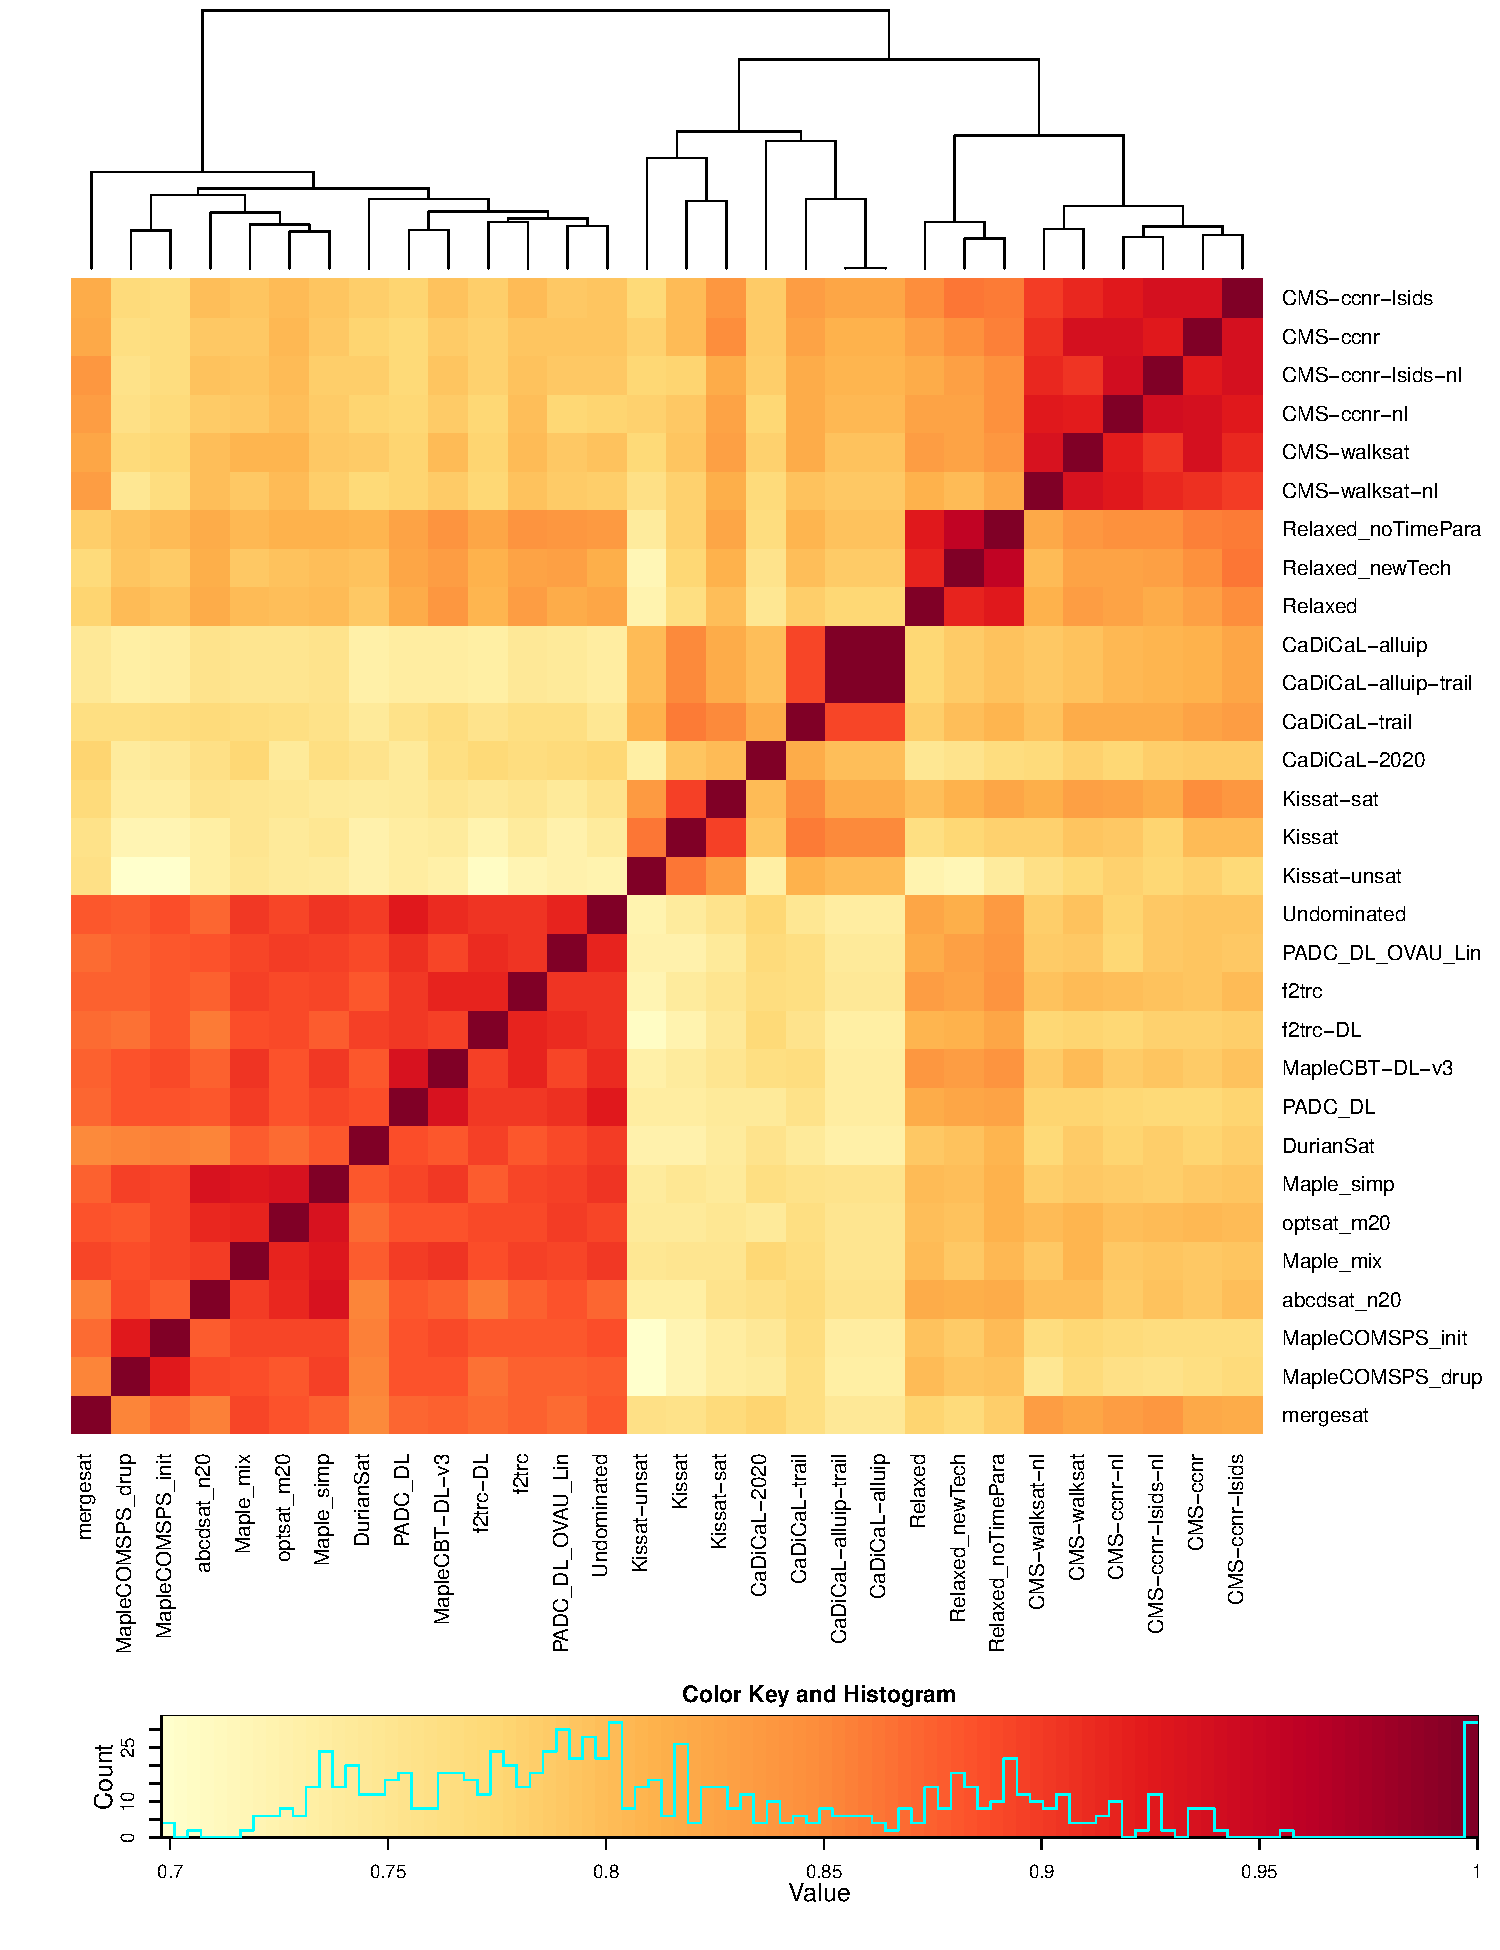
\includegraphics[width=\linewidth]{similarity/cross.pdf}
    \caption{Heat-map and dendrogram (top) based on the runtime similarity of the solvers participating in the main track.
      % Similarity is defined as
      % one minus the average taxicab distance normalized to the interval [0,1].
      % Spearman's rank correlation coefficient.
      Darker regions mean that the solvers are more similar.
      A more precise relation between color and similarity-value together with a histogram of the values that appear is given at the bottom.
    }
    \label{fig-similarity-main}
\end{figure}

% To estimate the similarity between the performance of the solvers of the Main
% Track we define a similarity metric $s$.
% identify each solver with a point in the 600-dimensional real vector
% space. Each component describes the PAR-2 runtime on one instance. We map the
% taxicab distance to the $[0, 1]$ interval and then to determine how similar two
% solvers are.


\subsection{Observations}

\paragraph{Marginal Contributions to VBS} Interestingly, the second (Relaxed-Maple-newTech) and the third (CryptoMinisat-lsids) ranked solver both outperform the winning solver (Kissat-sat) when we project only on the instance families ``antibandwidth''~\cite{} or ``timetable''~\cite{}. 


\section{Code-Bases and Winning Strategies}
\label{sec:analysis}

In the following we provide an overview on the participating teams and solvers,  and summarize new strategies which are implemented in the award winning solvers of this competition. 

We start with a few remarks on the evolution of code-bases of well known SAT solvers in Section~\ref{sec:codebases}. 
Our survey of the winning strategies in this competition starts with sequential (including incremental) SAT solving in Section~\ref{sec:part:seq}, then we continue with parallel SAT solving in Section~\ref{sec:part:par} and conclude with solvers in the cloud track in Section~\ref{sec:part:cloud}. 


\subsection{Code-Bases of SAT Solvers: ``On the Shoulders of Giants''}
\label{sec:codebases}

Progress in SAT solvers is usually recorded based on successful evaluations of  modifications of existing code-bases. 
One well-known tree of development is rooted in the code-base of \solver{Minisat} by Eén and Sörenson~\cite{Niklas:2003:Minisat}. 
A well-known fork of \solver{Minisat} is \solver{Glucose} by Audemard and Simon~\cite{Audemard:2018:Glucose}, among others introducing Literal Block Distance (LBD) for weighing clauses in forgetting heuristics~\cite{Audemard:2009:Glucose}. 
The SAT solver \solver{RISS} by Manthey is a successful and award winning fork of \solver{Glucose} in combination with the state-of-the-art preprocessor \solver{Coprocessor}~\cite{Manthey:2012:Coprocessor2}. 

Another more recent string of development is rooted in the \solver{CoMinisatPS} fork of \solver{Minisat} by Chanseok Oh introducing three-tier clause-managment~\cite{Oh:2015:satunsat}. 
The SAT solver \solver{Maple} appeared as a series of forks presenting innovative branching heurstics at SAT Competition 2016~\cite{Liang:2016:LRB}. 
The then award winning variant \solver{MapleCOMSPS} is an implementation of a hybrid branching heuristic of classic Variable-State Independend Decaying Sum (VSIDS) and the new Learning-Rate based Branching (LRB) in \solver{CoMinisatPS}~\cite{Liang:2016:MapleCOMSPS}. 

In SAT Competition 2017, Luo et al. integrated learnt clause minimization based on unit propagation (\solver{LCM}) in their award winning \solver{Maple\_LCM\_Dist}~\cite{Luo:2017:LCM} which also uses the new branching heuristic \solver{Distance (Dist)} in an initial solving period~\cite{Xiao:2017:MapleLCMDist}. 
Using \solver{Maple\_LCM\_Dist}, Ryvchin and Nadel successfully integrated conditional chronological backtracking (\solver{ChronoBT})~\cite{Nadel:2018:CBT}. 
They presented their award winning \solver{Maple\_LCM\_Dist\_ChronoBT} to SAT Competition~2018~\cite{Ryvchin:SC2018:MapleChronoBT}. 

Kochemazov et al. improved three-tier clause-management by persting additional clauses through hash-based detection of repeatedly learned clauses and presented their award winning~\solver{MapleLCMDistChronoBT-DL} to SAT Race~2019~\cite{Kochemazov:SC2019:MapleChronoBTDL}. 
As can be seen in Table~\ref{tab:solvers-incremental}, numerous submissions to SAT Competition~2020 are forks of some recently award winning \solver{Maple} solver. 

Starting as a \solver{Minisat}-fork and the integration of special xor treatment~\cite{Soos:2009:Crypto}, \solver{CryptoMinisat} by Soos continues to be a state-of-the-art and feature-rich SAT solver. 
One highlight of \solver{CryptoMinisat} is its advanced data-logging capabilities for statistical analysis of SAT solver behavior~\cite{Soos:2019:ChrystalBall}. 
In its new version~5, \solver{CryptoMinisat} has once again been award winning in SAT Competition~2020 (see Section~\ref{sec:cryptominisat}). 

Many independent and award-winning code-bases can be found among the state-of-the-art SAT solvers written by Biere. 
The sequential SAT solver \solver{Lingeling} has been award winning since SAT Competition~2011 and is still competitive in its parallel version \solver{Plingeling}~\cite{Biere:2012:Lingeling}. 
As of SAT Competition~2017, \solver{CaDiCaL} by Biere is another independent award winning and structured implementation of the state-of-the-art in SAT solving. 
Its improved reimplementation \solver{Kissat} won in several of this competitions sequential tracks by a large margin~\cite{Biere:SC2020}. 

The sequential variant of the \emph{new code-base} \solver{ParaFrost} by Osama and Wijs was submitted for the first time in this competition and introduced several interesting new concepts~\cite{Osama:SC2020:Parafrost}. 


\subsection{Sequential SAT Solving}
\label{sec:part:seq}

Sequential SAT solvers have been evaluated in the Main tracks as well as in the Incremental track of SAT Competition~2020. 
A total of $18$ teams submitted correct solvers to the Main track of the competition. 
Table~\ref{tab:solvers-main} displays an overview of the participating teams, base solvers and their variants. 
The recent genealogy of all submissions, is highlighted by \emph{base solver} and \emph{variant} columns. 
Underlined text is used to point out the important parts of the respective submissions name.

\renewcommand{\solver}[1]{\underline{\texttt{#1}}}
\newcommand{\solbert}[1]{\texttt{#1}}

\begin{table}[ht!]
\smaller
\arrayrulecolor{gray}
\centering
\begin{tabular}{|l|l|l|l|}
\hline
\bf Team & \bf Base Solver & \bf Variant / Name & \bf Award \\
\hline

\multirow{3}{*}{Biere} & \multirow{3}{*}{\solver{Kissat}} &  -- & \firsto, \firstu\\
 &  &  \solbert{sat} & \firsto, \firstu, \seconds\\
 &  &  \solbert{unsat} & \firstu, \thirdp\\
\hline
 Biere, Fleury &  \solbert{Cadical} & \solver{SC2020} & \\
\hline
 
\multirow{3}{*}{Zhang, Cai}
    & \multirow{3}{*}{\solbert{MapleLCMDistCBT-DL}} & \solver{Relaxed} & \\
 &  & \solbert{Rel. noTimeParam} & \\
 &  & \solbert{Rel. newTech} & \secondo, \firsts\\
\hline

\multirow{2}{*}{\stack{Soos, Cai, Devriendt, }{Gocht, Shaw, Meel}}~
 &  \multirow{2}{*}{\solbert{CryptoMiniSat-CCAnr}} &  -- & \thirdo, \thirds, \secondp\\
 &  &  \solbert{lsids} & \thirdo, \thirds, \secondp\\
\hline

\stack{Soos, Selman, Kautz, }{Devriendt, Gocht}~ & \solbert{CryptoMiniSat-WalkSAT} & -- & \\
\hline

\multirow{4}{*}{\stack{Hickey, Feng, }{Bacchus}}
 &  &  \solbert{trail} & \secondu\\
 &  &  \solbert{alluip} & \secondu, \firstp\\
 & \multirow{-3}{*}{\solbert{CaDiCaL}} &  \solver{alluip-trail} & \secondu, \firstp\\
 \cline{2-4}
 & \solbert{MapleLCMDist} & \solbert{alluip-trail} & \\
\hline

\multirow{3}{*}{Kochemazov} & \multirow{2}{*}{\solbert{MapleLCMDistCBT}} & \solver{f2trc} & \thirdu\\
 & & \solbert{f2trc-s} & \thirdu\\
 \cline{2-4}
 & \solbert{MapleLCMDistCBT-DL} & \solbert{f2trc} & \thirdu\\
\hline

\stack{Kochemazov, Zaikin, }{Kondratiev, Semenov} ~& \solver{MapleLCMDistCBT-DL-v3} & -- & \\
\hline

\multirow{4}{*}{\stack{Lonlac, }{Nguifo}}
 & \multirow{4}{*}{\solbert{MapleLCMDistCBT-DL-v3}} & \solver{Undominated} & \\
 &  & \solbert{Undom. Top16} & \\
 &  & \solbert{Undom. Top24} & \\
 &  & \solbert{Undom. Top36} & \\
\hline

\multirow{4}{*}{\stack{Tchinda, }{Djamegni}}
 & \multirow{4}{*}{\solver{Ex}\solbert{MapleLCMDistCBT}} & \solbert{padc\_dl} & \\
 &  & \solbert{padc\_dl\_ovau\_lin} & \\
 &  & \solbert{padc\_dl\_ovau\_exp} & \\
 &  & \solbert{psids\_dl} & \\
% \cline{2-3}& Glucose 3.0 & upGlucose-3.0\_PADC\\
\hline

Shaw, Meel & \solbert{MapleLCMDistCBT-DL-v3} & \solver{DurianSat} & \\
\hline

\multirow{2}{*}{Chen}
 & \multirow{2}{*}{\solbert{MapleLCMDistCBT-DL}} & \solver{Maple\_Mix} & \\
 &  & \solver{Maple\_Simp} & \\
\hline

Riveros & \solbert{MapleLCMDistCBT} & \solver{SLIME} & \\
\hline

\multirow{3}{*}{Li, Wu, Xu, Chen}
 & \multirow{3}{*}{\solbert{MapleLCMDistCBT-DL}} & \solver{Scavel} & \\
 &  & \solbert{Scavel01} & \\
 &  & \solbert{Scavel02} & \\
\hline

\multirow{2}{*}{\stack{Liang, Oh, Nejati, }{Poupart, Ganesh}}
 & \multirow{2}{*}{\solver{MapleCOMSPS\_LRB\_VSIDS\_2}} & -- & \\
 &  & \solbert{init} & \\
\hline

\multirow{4}{*}{\stack{Chowdhury, }{Müller, You}}
 & \multirow{4}{*}{\solbert{MapleLCMDistCBT-DL-v2.2}} & \solver{exp}\solbert{-V-LGB} & \\
 &  & \solbert{exp-V-L} & \\
 &  & \solbert{exp-L} & \\
 &  & \solbert{exp-V} & \\
\hline

\multirow{4}{*}{\stack{Li, Luo, Xiao, }{Li, Manyà, Lü}}
 & \multirow{4}{*}{\solver{MapleCM}} & \solver{+dist} & \\
 &  & \solbert{+dist+sattime2s+-} & \\
 &  & \solbert{+dist+simp2--} & \\
 &  & \solbert{used+dist} & \\
\hline

Kaiser, Hartung & \solbert{MapleLCMDist} & \solver{PauSat} & \\
\hline

\multirow{2}{*}{Osama, Wijs} 
 & \multirow{2}{*}{\solver{ParaFROST}} & -- & \\
 &  & \solbert{CBT} & \\
\hline
\end{tabular}
\caption[Teams and Solvers in the Main Tracks]{Teams and Solvers in the Main Tracks: Column~2 highlights the recent genealogy of submissions and Column~3 displays configuration names as well as names of forks. We partially \solver{underlined} submission names. Awards in the Main- (M), Planning- (P), Sat- (s), and Unsat- (u) Tracks are indicated by a string TX with $T \in \{M, P, s, u\}$ and $X \in \{1,2,3\}$. }
\label{tab:solvers-main}
\end{table}

\renewcommand{\solver}[1]{\texttt{#1}} % sorry ;)

%%%%%%%%%%%%%%%%%%%%%%%%%%%%%%%%%%%%%%%%%%%%%%%%%%

Four submissions made it to participate in the Incremental Library track, some of which, e.g, \solver{CryptoMinisat-5}, have also been evaluated and awarded in the Main sequential track. 
Submissions to the Incremental Library track have been evaluated with respect to $6$ different applications -- each with $50$ benchmark instances. 
Table~\ref{tab:solvers-incremental} displays an overview of the participating teams and solvers. 
In this table, \emph{Score} denotes the number of application categories in which the solvers won based on their PAR-2 score. 

\begin{table}[ht]
\smaller
\arrayrulecolor{gray}
\centering
\begin{tabular}{|l|l|c|}
\hline
\bf Team & \bf Solver & \bf Score\\
\hline
\stack{Soos, Cai, Devriendt, }{Gocht, Shaw, Meel}~ & Cryptominisat-5 & 3 \\
\hline
\stack{Biere, Fleury}~ & CaDiCaL-sc2020 & 1 \\
\hline
Chen & abcdsat-i20 & 1 \\
\hline
Manthey & Riss-7.1.2 & 1 \\
\hline
\end{tabular}
\caption[Teams and Solvers in the Incremental Track]{Teams and Solvers in the Incremental Library Track: Score indicates the amount of application categories won with the submission.}
\label{tab:solvers-incremental}
\end{table}


\subsubsection{Kissat} 

Three major configurations of \solver{Kissat} were evaluated in this competition. 
That includes one default configuration and two specialized configurations which are specifically tailored towards satisfiable and unsatisfiable instances, respectively. 
\solver{Kissat} won \emph{four awards}, by achieving first place in the Main track, first place in the Unsat track, second place in the Sat track and third place in the Planning track. 

\solver{Kissat} is a reimplementation of \solver{CaDiCaL} in C,
but comes with new sophisticated lazy data-structures for clause state monitoring, e.g., through binary clause inlining, sentinel values and bit stuffing~\cite{Biere:SC2019,Biere:SC2020}. 
Moreover, forward subsumption for learned clauses is mostly replaced by vivification algorithms~\cite{ChuMinLi:2020:Vivification}. 

\solver{Kissat} uses a new unit (``ticks'') to measure the length of two alternating restart-modes based on the approximate number of cache-line accesses, after conflict-rate has been obeserved to be too unstable for the use-case~\cite{Biere:SC2020}. 

\solver{Kissat} also exploits an innovative use-case for autarkies to account for saved phases. 
In order to keep valuable information of saved phases, before each rephasing step, \solver{Kissat} computes the largest autarky for the assignment implied by the current saved phases~\cite{Kiesl:2019:Autarkies}. 
As such an autarky might contain satisfying assignments which imply disconnected components, those variables are subject to subsequent variable elimination. 


\subsubsection{CryptoMiniSat-CCAnr and CryptoMiniSat5}
\label{sec:cryptominisat}

\solver{CryptoMinisat} won \emph{four awards}, two third places in the Main and Sat tracks, one second place in the Planning track, and first place in the Incremental Library track. 
Two submitted variants \solver{default} and \solver{LSIDS} scored mostly adjacent ranks in the evaluation of tracks. 
The \solver{LSIDS} variant of \solver{CryptoMinisat} comes with a new hybrid phase selection approach~\cite{Shaw:2020:LSIDS,Soos:SC2020}.

\solver{CryptoMinisat} comes with an independent implementation of the recent hybrid branching heuristic which alternates between classic phase saving and target phase selection~\cite{Biere:SC2019}.

\solver{CryptoMiniSat-CCAnr} integrates stochastic local search (SLS) in a unique way~\cite{Cai:2015:CCAnr}. 
\solver{CryptoMiniSat-CCAnr} regularly schedules short periods of local search and imports the best assignment found by the SLS solver for phase selection -- a procedure which is known as ``rephasing'' from CaDiCaL~\cite{Biere:SC2019}.
In addition, \solver{CryptoMiniSat-CCAnr} bumps the VSIDS scores of the first 100 variables in those clauses which the SLS solver weighs most hard to satisfy~\cite{Soos:SC2020}.

Inprocessing has been extended to include ternary resolution and more vivification~\cite{ChuMinLi:2020:Vivification}. 
All the new features are fully supported in \emph{incremental} mode. 
\solver{CryptoMinisat} alternates decay factors of its branching heuristics, thus avoiding the restriction to a ``single best'' configuration~\cite{Soos:SC2020}. 
The submitted version of \solver{CryptoMinisat} entails a new optimized implementation of Gauss-Jordan Elimination~\cite{Soos:2020:CNFXOR}. 
\solver{CryptoMinisat} periodically executes the \solver{BreakId} algorithm to  calculate symmetry breaking clauses~\cite{Devriendt:2016:BreakId}.


\subsubsection{Trail Saving and Stable AllUip in CaDiCaL}

Based on \solver{CaDiCaL}, its variants \solver{Trail} and \solver{AllUip} present implementations of a new \emph{Trail Saving} approach~\cite{Hickey:2020:TrailSaving} and improved clause-learing based on the notion of \emph{Stable AllUIP}~\cite{Bacchus:SC2020}. 
Submitted were the three variants \solver{Trail}, \solver{AllUip} and \solver{AllUip+Trail}. 
The variants including \emph{Stable AllUIP} were the most successful and won the first price in the Planning Sub-Track. 

The \emph{Stable AllUip} variants resolve additional clauses beyond the 1st Unit Implication Point (1-UIP) and keep them if they are of smaller size or LBD than the 1-UIP clause. 
By monitoring the frequency of clauses which successfully pass that filter, the solver dynamically limits the amount of attempts~\cite{Zhang:2001:ClauseLearning,Bacchus:SC2020}.
The \emph{Trail Saving} variant caches backtracked portions of the trail and uses them to restore decision levels during search if possible~\cite{Hickey:2020:TrailSaving}. 


\subsubsection{Relaxed Maple newTech}

The \solver{Relaxed} fork of \solver{MapleLCMDistCBT-DL} was first presented to the community in SAT Race 2019~\cite{Xindi:SC2019}. 
In SAT Competition~2020, its new variant \solver{newTech} showed a good performance especially on satisfiable instances. 
The solver won two awards, the second price in the Main track and the first price in the Sat track.

The \solver{Relaxed} fork integrates short runs of the local search solver \solver{CCAnr} through periodic ex- and import of assignments~\cite{Xindi:SC2019}. 
The submitted versions of \solver{Relaxed Maple} use a probabilistic schedule for switching between $10$ phase selection modes. 
The award winning variant \solver{newTech} uses occurrence counts of variables in unsatisfied clauses during SLS runs to recalculate variable priorities for their modified branching heuristic~\cite{Xindi:SC2020}. 


\subsubsection{Maple F2TRC}

The \solver{F2TRC} fork of \solver{MapleLCMDistCBT} won the third price in the Unsat track. 
\solver{F2TRC} comes with a deterministic reimplementations of former winning strategies, e.g., by replacing time intervals by conflict intervals~\cite{Kochemazov:SC2020}. 

\solver{F2TRC} introduces an improved management of learned clauses in the tree tiers \emph{core}, \emph{tier2} and \emph{local} which are inherited from \solver{CoMinisatPS}~\cite{Oh:2015:satunsat}.
A dynamic size limit for the \emph{core} tier, triggers the reassignment of inactive clauses from \emph{core} to \emph{tier2}. 
To conter-act an observered starving of tier2, the conflict-based heuristic that controls demotion of clauses from \emph{tier2} to \emph{local} was replaced by a size based heuristic~\cite{Kochemazov:SC2020}. 


\subsection{Parallel SAT Solving: Winners of the Parallel Track}
\label{sec:part:par}

\begin{table}[b]
\smaller
\centering
\begin{tabular}{|l|l|l|}
\hline
\bf Team & \bf Solver & \bf Awards\\
\hline
\multirow{2}{*}{\stack{Vallade, Le Frioux, Baarir, }{Sopena, Kordon}}~
 & P-MCOMSPS-STR-32 & \firsto \firsts \secondu \\
 & P-MCOMSPS-STR-64 & \firsto \\
\hline
\multirow{2}{*}{\stack{Biere, Fazekas, }{Fleury, Heisinger}}
 & Plingeling & \secondo \thirds \firstu \\
 & Treengeling & \\
\hline
\multirow{2}{*}{Nabeshima, Inoue}
 & ManyGlucose-32 & \thirdo \thirdu \\
 & ManyGlucose-64 & \thirdu \\
\hline
\multirow{2}{*}{Tchinda, Djamegni}
 & painlessmaplevone & \seconds \\
 & painlessmaplevtwo & \seconds \\
\hline
Li, Wu, Xu, Chen & syrupscavel & \\
\hline
Chen & abcdsatptwenty & \\
\hline
\end{tabular}
\caption{Teams and Solvers participating in the parallel track.}
\end{table}

\subsubsection{P-MCOMSPS-STR} 

P-MCOMSPS-STR is built from the Painless framework~\cite{Frioux:2017:Painless} for solver parallization and uses the MapleCOMSPS solver~\cite{Liang:2017:Maplecomsps} as a building block. 
The authors submitted a 32 and 64 core version and won 3 awards, first place in the overall ranking, first place in the SAT ranking and second in the UNSAT ranking. 
The 64 core version performed slightly worse than the 32 core version in the overall ranking, and that gap is bigger for the SAT-only ranking and worst for the UNSAT-only ranking, such that in the separate rankings only the 32 core version is responsible for winning the prices. 

The painless framework uses a generic interface to integrate a solver and abstracts away the implementation details of parallelism and concurrenct data-structures, such that implementations within the framework boil down to implementing parallelization and clause sharing strategies. 

In the submitted version of P-MCOMSPS-STR, diversification is done via diverse fixed configurations of branching strategies (LRB and VSIDS) and sparse random intialization of variable polarities like in~\cite{Balyo:2015:Hordesat}. 
One instance of their ``sequential engines'' performs concurrent clause strengtheing as described in~\cite{Wieringa:2013:CCS} and another single instance is configured to perform Gaussian eliminiation during preprocessing. 

For sharing they use an all-to-all strategy with a regular exchange of a fixed size buffer and a dynamic clause lbd limit. 


\subsubsection{Plingeling} 

Plingeling got three awards, first place in the Unsat Category, third place in Sat and second place in the overall evaluation. 
Plingeling is an extension of the well-known SAT solver Lingeling~\cite{} and did not change since 2016. 
Via a global master queue, Plingeling shares unit clauses, equivalences and short clauses with clauses with at most 40 literals and glucose LBD level of at most 8 and random seeds, e.g., for diversification via default polarities.~\cite{} 


\subsubsection{ManyGlucose}

The authors of ManyGlucose received two awards in this competition. 
ManyGlucose was submitted in 32-core and 64-core variants~\cite{}.
The 32-core variant won two third prices, one in the overall evaluation and one in the unsat sub-track. 
ManyGlucose is a fork of GlucoseSyrup~\cite{} and uses strategies similar to those known from ManySAT~\cite{} in order to achive deterministic solver runs. 


\subsubsection{Painless Maple} 

The authors Painless Maple received one award for second best performance in the Sat sub-track of the parallel track. 
However, the solver was last in the Unsat sub-track. 

The authors implemented a couple of modifications (\todo{name them}) on top of the MapleLCMDistChronoBT~\cite{} solver, which they also submitted in various configurations to the main track. 
The two submissions in the parallel track use painless as a parallelization framework. 

Their sharing strategy includes splitting their workers into two categories, where the solvers in the first category only export clauses and only solvers in the second category import and export clauses. 

They submitted two variants with different diversification strategies. 
In their first variant they use different configurations of configurations of the newly implemented strategies. 
The second variant uses a more classic diverisification strategy by randomizing polarities and variable scores. 


\subsection{Massively Parallel SAT Solving: Winners of the Cloud Track}
\label{sec:part:cloud}

\begin{table}[ht]
\smaller
\centering
\begin{tabular}{|l|l|l|}
\hline
\bf Team & \bf Solver & \bf Rank\\
\hline
Schreiber & mallob-mono & 1\\
\hline
\stack{Ehlers, Kulczynski, }{Nowotka, Sieweck}~ & TopoSAT2 & 2\\
\hline
Riveros & Slime & 3\\
\hline
\multirow{2}{*}{\stack{Biere, Fazekas, }{Fleury, Heisinger}}~ & Paracooba & -\\
& Paracooba-March & -\\
\hline
Hartung & CTSat & -\\
\hline
\end{tabular}
\caption{Teams and Solvers participating in the cloud track.}
\end{table}


\subsubsection{Mallob Mono}

The massively parallel SAT solver Mallob is based on HordeSAT~\cite{}. 
Mallob is a framework for massivley parallel and distributed \emph{malleable job scheduling}, and thus can perform dynamic load balancing on many jobs of varying priorty.
However, in the submitted version Mallob Mono, this functionality is disabled, as traditionally in SAT Competition all resources are busy solving one single instance only. 

Mallob uses the the 2018 version \emph{bcj} of Lingeling~\cite{} and employs diversification via randomized sparse initialization of branching scores just like it is done in Plingeling~\cite{}. 
Every 14th process, however, runs the local search solver YalSAT~\cite{}. 

Clause exchange is handled considerably different from previous approach. 
Workers are organized in a binary tree and clauses are asynchronously aggregated in a buffer which is passed along this tree from leafs to the root. 
Each node performs a three way merge of the local and the two incoming buffers. 
Only the final aggragate at the root of that binary tree is broadcast to all the solvers. 

To limit sharing, there is a global size limit of $5$ for all the shared clauses. 
The buffer has a limited size as well, but that size depends on the position in the binary tree, with root having the largest buffer and leaves the smallest. 
Clauses are sorted by there size during aggregation, such that smaller clauses are preferred over longer clauses. 
Duplicates are filtered out using a bloom filter, which is cleared periodically. 
There is a special filter for duplicate unit-clause which especially useful during startup. 


\subsubsection{TopoSAT 2}

TopoSAT~2 is a massively parallel SAT solver using Glucose~3 with lockfree clause-exchange as in ManySAT~\cite{} on each node, and using MPI to share clauses between nodes. 

In Toposat~2, diversification is done via different strategies used for branching, restarting and clause forgetting. 
Clauses are strengthened before they are exported. 
Locally, clause import is delayed until the local trail-size is low in a monitored period. 


\subsubsection{Slime}

Slime is build on top of MapleLCMDistChronoBT and was first submitted to SAT Race 2019 suggesting the new phase selection heuristic~\cite{}. 
The 2020 version apparently adds some kind of periodic randomization in geometrically increasing intervals~\cite{}. 
Even thought the sequential solver was unsuccessful in the Main Track, its MPI-based cloud version, won the third price in this competitions cloud track. 


\section{Conclusion and Prospects}
\label{sec:conclusion}

\todo{Summarize Winning Strategies}

\todo{Ideas for Future Competitions}

\section*{Acknowledgements}
Martin Suda was supported by the ERC Consolidator grant AI4REASON no. 649043 under the EU-H2020 programme,
the Czech Science Foundataion project 20-06390Y, and the project RICAIP, no. 857306 under the EU-H2020 programme.

\bibliographystyle{elsarticle-num}
\bibliography{main}

\end{document}
